\section{Réseaux de neurones}

\subsection{Introduction}

Les réseaux des neurones représentent une des méthodes les plus utilisées en \textit{Machine Learning}, ils sont utilisés dans de nombreux domaines comme la vision par ordinateur entre autres. Leur popularité vient du fait qu'ils permettent de modéliser des problèmes très complexes. Récemment le champion du monde au jeu de Go vient de subir une défaite il y a deux semaines par un réseau de neurones\footnote{AlphaGo développé par Google}, dans le jeu que les informaticiens considèrent comme étant l'un des jeux les plus durs à automatiser puisque le nombre de possibilités énorme.
Cette méthode nécessite néanmoins une puissance de calcul et une mémoire assez conséquente, dès que le nombre des noeuds commencent à croitre.

\newpage

\subsection{Structure du réseau}

Un réseau de neurons peut etre representé comme suit :

\def\layersep{2.5cm}

\begin{figure}[h]
\centering
    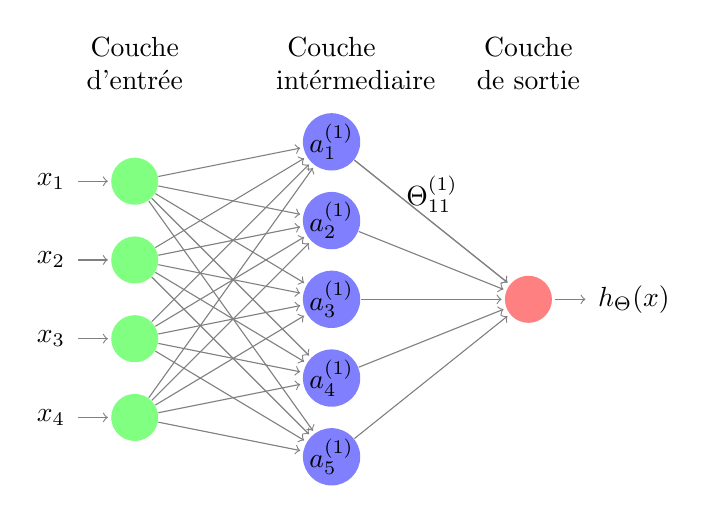
\begin{tikzpicture}[shorten >=1pt,->,draw=black!50, node distance=\layersep]
        \tikzstyle{every pin edge}=[<-,shorten <=1pt]
        \tikzstyle{neuron}=[circle,fill=black!25,minimum size=17pt,inner sep=0pt]
        \tikzstyle{input neuron}=[neuron, fill=green!50];
        \tikzstyle{output neuron}=[neuron, fill=red!50];
        \tikzstyle{hidden neuron}=[neuron, fill=blue!50];
        \tikzstyle{annot} = [text width=4em, text centered]

        % Draw the input layer nodes
        \foreach \name / \y in {1,...,4}
        % This is the same as writing \foreach \name / \y in {1/1,2/2,3/3,4/4}
            \node[input neuron, pin=left: $x_\y$] (I-\name) at (0,-\y) {};

        % Draw the hidden layer nodes
        \foreach \name / \y in {1,...,5}
            \path[yshift=0.5cm]
                node[hidden neuron] (H-\name) at (\layersep,-\y cm) {$a_\y^{(1)}$};

        % Draw the output layer node
        \node[output neuron,pin={[pin edge={->}]right:$h_\Theta(x)$}, right of=H-3] (O) {};

        % Connect every node in the input layer with every node in the
        % hidden layer.
        \foreach \source in {1,...,4}
            \foreach \dest in {1,...,5}
                \path (I-\source) edge (H-\dest);

        % Connect every node in the hidden layer with the output layer
        \path (H-1) edge node[above]{$\Theta_{11}^{(1)}$} (O);
        \foreach \source in {1,...,5}
            \path (H-\source) edge (O);

        % Annotate the layers
        \node[annot,above of=H-1, node distance=1cm] (hl) {Couche intérmediaire};
        \node[annot,left of=hl] {Couche d'entrée};
        \node[annot,right of=hl] {Couche de sortie};
    \end{tikzpicture}
    \caption{Exemple d'un reseau de neurones}

\end{figure}
La couche d'entrée est ce qui est fourni au programme. Dans le cas d'une vision par ordinateur cela pourrait être les pixels de l'image, dans le cas d'un filtre à spam, cela pourrait être des booléans représentant l'existence de certains mots-clés.

Les couches intermédiaires permettant de complexifier le réseau et de lui permettre de modéliser des problèmes de plus en plus complexes, le souci est qu'elles augmentent énormément le temps de calcul.

La couche de sortie représente le résultat retourné par le réseau qui est un vecteur de booléans (souvent il est de taille 1) qui nous informe si oui ou non le vecteur d'entrée appartient à une classe donnée (par exemple si une image fournie en entrée est une voiture, ou si un message est un spam ).

Le vecteur $a^{(1)} = \begin{pmatrix}
  a_1^{(1)}  \\
  a_2^{(1)}  \\
  a_3^{(1)}  \\
  a_4^{(1)}  \\
  a_5^{(1)}  \\
 \end{pmatrix}$
permets de calculer la sortie $h_\Theta(x)$, en effet on pourrait considérer le vecteur $a^{(1)}$ comme la nouvelle entrée est ainsi de suite. Ce procédé s'appelle la \textit{Forward Propagation}.

Les poids sont stockés dans une matrice tridimensionnelle notée $\Theta$, chaque poids est dénoté par : $\Theta_{ij}^{(k)}$ où $k$ est le numéro de la couche, $i$ le numéro du noeud de la couche 2 et $j$ le numéro du noeud de la couche 1.

On peut alors calculer $h_\Theta(x)$ comme suit :

\begin{gather*}
    z_1^{(1)} = \Theta_{11}^{(0)}x_1 + \Theta_{12}^{(0)}x_2 + \Theta_{13}^{(0)}x_3 + \Theta_{14}^{(0)}x_4\\
    a_1^{(1)} = g(z_1^{(1)})\\
    z_2^{(1)} = \Theta_{21}^{(0)}x_1 + \Theta_{22}^{(0)}x_2 + \Theta_{23}^{(0)}x_3 + \Theta_{24}^{(0)}x_4\\
    a_2^{(1)} = g(z_2^{(1)})\\
    z_3^{(1)} = \Theta_{31}^{(0)}x_1 + \Theta_{32}^{(0)}x_2 + \Theta_{33}^{(0)}x_3 + \Theta_{34}^{(0)}x_4\\
    a_3^{(1)} = g(z_3^{(1)})\\
    z_4^{(1)} = \Theta_{41}^{(0)}x_1 + \Theta_{42}^{(0)}x_2 + \Theta_{43}^{(0)}x_3 + \Theta_{44}^{(0)}x_4\\
    a_4^{(1)} = g(z_4^{(1)})\\
    z_5^{(1)} = \Theta_{51}^{(0)}x_1 + \Theta_{52}^{(0)}x_2 + \Theta_{53}^{(0)}x_3 + \Theta_{54}^{(0)}x_4\\
    a_5^{(1)} = g(z_5^{(1)})\\
    h_\Theta(x) = g(\Theta_{11}^{(1)}a_1 + \Theta_{12}^{(1)}a_2 + \Theta_{13}^{(1)}a_3 + \Theta_{14}^{(1)}a_4)\\
\end{gather*}

Ce procédé est communement appelé : \textit{Forward Propagation}.

Ici la fonction $g(x)$ est ce que l'on désigne une fonction d'activation, dans le programme nous avons choisi la fonction de \textit{Sigmoid}\footnote{https://fr.wikipedia.org/wiki/Sigmo\%C3\%AFde\_\%28math\%C3\%A9matiques\%29} (ce choix pourra être changé dans le futur), il existe une multitude de fonctions, notre choix est basé sur celui fait par \textit{Andrew}.
La fonction \textit{Sigmoid} est définie par : $g(x) = \frac{1}{1 + e^{-x}}$ dont la courbe est :

\begin{figure}[h]
\centering
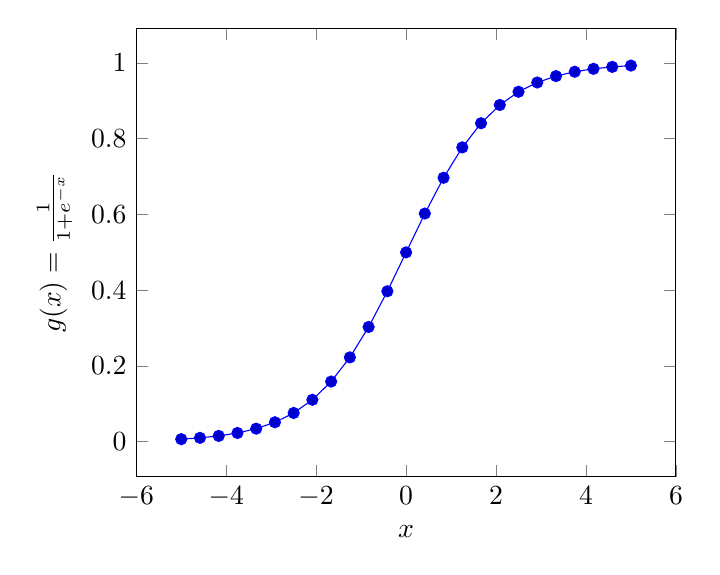
\begin{tikzpicture}
  \begin{axis}[
    xlabel=$x$,
    ylabel={$g(x) = \frac{1}{1 + e^{-x}}$}
  ]
    \addplot {1 / (1 + exp(-x))};
  \end{axis}
\end{tikzpicture}
\caption{Courbe de la fonction Sigmoid}
\end{figure}

Cette fonction a la particularité de converger très vite vers 1 ou 0 ce qui s'avère très utile puisque le résultat final doit être un booléan.

\subsubsection{Fonction du cout}

La fonction du cout permet de mesurer à quel point notre réseau est précis, cette fonction dépend de $\Theta$ et la minimiser permettera d'augmenter la précision de notre réseau.

Cette fonction est définie par :

\begin{equation}
J(\Theta) = -\frac{1}{m}[\sum\limits_{i=0}^m\sum\limits_{k=0}^K y_k^{(i)}log(h_\theta(x^{(i)})_k) + (1 - y_k^{(i)})log(1 - h_\theta(x^{(i)})_k)] + \frac{\lambda}{2m}\sum\limits_{l=0}^{L - 1}\sum\limits_{i=0}^{s_l}\sum\limits_{j=1}^{s_l + 1}(\Theta_{ij}^{(l)})^2
\end{equation}

Avec :

\begin{description}

\item[$m$ : ] Taille du dataset donnée en entrée (pour l'entrainement du classificateur).
\item[$K$ : ] Taille du vecteur de sortie.
\item[$y$ : ] Réponse à une donnée particulière par exemple 1 si l'image en entrée est une voiture.
\item[$h_\theta(x^{(i)})$ : ] Réponse donnée par le réseau de neurons (n'est pas nécéssairement égale à y).
\item[$\lambda$ : ] : Parametre fournie par l'utilisateur qui permet d'éviter \textit{l'overfitting\footnote{L'overfitting est le fait d'avoir un réseau qui fournit d'excellents réseultats sur le dataset d'entrainements mais a des performences médiocres sur des données qu'il n'a jamais vu}}.
\item[$L$ : ] Nombre de couches.
\item[$s_l$ : ] Nombre de noeuds dans la couche l.

\end{description}

Entrainer le réseau des neurones revient donc à trouver le $\Theta$ qui minimisera la fonction, cela se fera grace à des fonctions pré fournies par la bibliothèque \textit{Dlib}.
Il faut tout de même noter qu'en général cette fonction n'est pas convexe\footnote{https://stats.stackexchange.com/questions/106334/cost-function-of-neural-network-is-non-convex}, l'algorithme de minimisation ne garantit donc en rien qu'on trouvera un minima global, en fait trouver un minimum global serai un problème NP-difficile\footnote{Reference: Avrim Blum and Ronald L. Rivest, "Training a Three-Neuron Neural Net is NP- Complete", Neural Networks 5(1) January 1992. [https://people.csail.mit.edu/rivest/pubs/BR93.pdf]} mais en pratique les minima locals peuvent donner des résultas satisfaisants si le réseau possède assez de couches intermédiaires\footnote{https://stats.stackexchange.com/questions/203288/understanding-almost-all-local-minimum-have-very-similar-function-value-to-the}.

Pour minimiser cette fonction nous utilisons le \textit{BFGS}, un algorithme quasi-newtonien\cite{analyse}. Cet algorithme est déja implémenté dans Dlib, et prends deux paramétres : une fonction et son gradient dans un point donné.

Pour calculer le gradient nous utiliserons un procédé nommé la \textit{Back Propagation}. Il faut noter qu'il est également possible d'approcher ce gradient par des méthodes numérique, cette dernière à l'avantage d'etre plus facile et plus rapide à implémenter mais elle est beaucoup plus couteuse et ne sera donc pas utilisée, ces méthodes numériques permettent tout de même de vérifier si une implémentation de la \textit{Back Propagation} est correcte, mais ne devra être utilisé que pour des fins de déboguage.

\newpage
\subsubsection{Back Propagation}

La \textit{Back Propagation} nous permettera de calculer les gradients de la fonction du cout.

\begin{algorithm}[H] %or another one check
 \caption{Back Propagation}
     \SetAlgoLined
	\SetKwProg{Fn}{Procedure}{}{}
	\Fn{backPropagation()}{
		Initialiser $\Delta_{ij}^{(l)} = 0$ pour tout $l$, $i$, $j$;\\
		\For{$i$ allant 1 à $m$}
	    {
	    	Calculer les différents $a^{(l)}$ par la forward propagation;\\
            Calculer $\delta^{(L)} = a^{(L)} - y^{(i)}$;\\
            \For{$l$ allant de L - 1 à 2}
            {
                $\delta^{(l)} = (\Theta^{(l)})^T\delta^{(l + 1)}.*\footnote{Multiplication élément par élément}g^{'}(z^{(l)})$
            }
            $\Delta_{kj}^{(l)} = \Delta_{kj}^{(l)} + a_j^{(l)}\delta_k^{(l + 1)}$\\
	    }
		$\frac{\partial}{\partial \Theta_{ij}^{(l)}}J(\Theta) = \frac{1}{m}\Delta_{ij}^{(l)} + \lambda\Theta_{ij}^{(l)}$ (si $j \neq 0$)\\
        $\frac{\partial}{\partial \Theta_{ij}^{(l)}}J(\Theta) = \frac{1}{m}\Delta_{ij}^{(l)}$ (si $j = 0$)\\
}
\textbf{Fin}
\end{algorithm}

Bien entendu la \textit{Back Propagation} ne permet de calculer les gradients que pour un point donnée, elle sera donc appelé plusieurs fois, c'est pour ca qu'opter pour un algorithme utilisant un nombre d'itérations faibles (contrairement à un gradient descendant par exemple) peut considérablement réduire le temps du calcul.

Une fois la fonction $J(\theta)$ minimisée, le réseau est, en théorie, capable de prédire des résultats juste via une simple forward propagation pour sur une entrée donnée. Il faut tout de meme garder en tête que minimiser la fonction $J(\theta)$ peut causer un problème d'overfitting, ce qui sera résolu par l'essaie de plusieurs valeurs de $\lambda$ (prametre optionnel du constructeur) pour le moment ZZBrain ne calcule pas le $\lambda$ optimal, ce qui signifie que l'utilisateur devra lui même choisir des valeurs et les tester.
